%% LyX 2.2.0 created this file.  For more info, see http://www.lyx.org/.
%% Do not edit unless you really know what you are doing.
\documentclass[english]{article}
\usepackage[T1]{fontenc}
\usepackage[latin9]{inputenc}
\usepackage{geometry}
\geometry{verbose,lmargin=3cm,rmargin=3cm}
\usepackage{amsmath}
\usepackage{graphicx}
\usepackage{setspace}
\onehalfspacing
\usepackage{babel}
\usepackage{cite}

\begin{document}

%\begin{quote}
%\begin{spacing}{0.5}
%\begin{center}
%{\footnotesize{}UNIVERSITY OF CALIFORNIA, DAVIS}\\
%{\footnotesize{} DEPARTMENT OF COMPUTER SCIENCE}
%\par\end{center}{\footnotesize \par}
%\end{spacing}
%\end{quote}

%\rule[0.5ex]{1\columnwidth}{1pt}

\title{\huge{Using AlphaGo Zero Techniques to Play Tic-Tac-Toe, Connect Four and Chess: Crop Dusting with an F-18}}
%\rule[0.5ex]{1\columnwidth}{1pt}
\author{
Adrian Chmielewski-Anders, Kenan Nabalt, Parsoa Khorsand, Sadegh Shams \\
\{achmielewski, kanalbant, pkhorsand, mshamsabardeh\}@ucdavis.edu
}
\date{}

\maketitle


\begin{abstract}
There has been much success with using deep neural networks combined
with various forms of tree search in order to play perfect knowledge, zero-sum
games. Most notable are the techniques of AlphaGo. However,
these techniques still rely on datasets of professional games for training.
Most recently, it has been demonstrated that it is possible to play Go at
the highest level, with no prior game datasets.
This is achieve through consolidating the policy and value networks into a single
network, and omitting the use of rollouts. This single policy and vlaue network
in conjunction with a modified Monte-Carlo Tree Search algorithm has proven to
yield exceptional results. We try to use this approach to play
other games, namely tic-tac-toe, Connect Four, and chess.

\end{abstract}

\section{Introduction}

The supervised learning is based on the data obtained from the experts.
These data are expensive to gather and sometimes unreliable. The best
performance that can be expected from a Neural Network being trained
with such data cannot exceed human level intelligence. Playing chess
based on supervised learning can achieve performance of the champions,
however, cannot perform better. 

On the other hand, the reinforcement learning systems can learn on
their own based on their experiences and by taking random actions.
This characteristic makes them capable of surpassing human knowledge.
Reinforcement learning has recently drawn attentions of researchers
and industries do to their promising capacities. These systems have
demonstrated better performance than human in some domains{[}ref{]}.
Training deep neural network with reinforcement learning have outperformed
human in computer games such as Atari and 3D virtual environments
{[}ref 8-10p{]}. There have been some efforts in the literature by
scholars to implement chess based on the reinforcement learning. In
{[}1,2,3{]} the authors propose the reinforcement learning for the
self-play and the training is done based on temporal difference learning.
The authors have used handcrafted input features and these features
can be the source of performance limitation. 1 and 2 deploy a pre-existing
computer programs as training opponents which limits the best achievable
performance. The large state space of the chess together with the
above-mentioned problems makes our team to mimic the AlphaGo Zero
algorithm, developed by Google Deep Mind for the Game of Go, as reasonable
solution to address these problems. This algorithm solves the problem
of large state space by exploring only those states that have more
probability of wining. To our best knowledge this is the first work
implementing AlphaGo Zero algorithm for the game of Chess. The following
sections of this paper are organized as follow: \dots . 

\section{Methods}

The majority of the method is taken from \cite{AlphaGoZero} although key pieces
are modified so as to allow the method to work for other games such as chess.
These differences are noted throughout.

\subsection{Holistic Model}

The goal is to build a system which will output which action $a$ to make at a
give game state $s_t$. To do this, a variant of Monte-Carlo Tree Search (MCTS)
is used wherein the neural
network $f_{\theta}$ is used to guide the search. In the initial
game tree, the root node $s_0$ has no children. Such a node (while having
children since there exists legal actions from this state) is referred to as a
leaf node, distinct from a terminal node (one where there does not exist any
legal action resulting in a next state). To make a move, the MCTS starts with a
tree of just one node. Since it is a leaf node, it is expanded. Its children,
that is the next legal states, are added to the tree after feeding the states
through the neural network and obtaining $(p, v) = f_{\theta}(s)$ where $p$ is a
vector of move probabilities and $v$ is a scalar representing the value of the
state. In our modified version, both are scalars and we achieve a vector of $v$
values by feeding a combination of the current state and next states into the
network, resulting in more than one call to $f_{\theta}$. The values $p$ and $v$
are propagated through the tree, and the search is repeated. The MCTS operation
walks down the tree and makes decisions as to where to go based upon $p$ and $v$
as well as the visit count $N$. After many searches, the MCTS returns a
probability distribution $\pi$ based on the move count $N$. Based on $\pi$ a
move is selected as the move to make.

MCTS may therefore be viewed as a policy enhancement operator. The goal of the
method is to create data via games of self-play and to train the network based
on the true policy, the result of many MCTS searches, and the true value, the
winner of the game. Repeating this in the policy
iteration procedure is the strength of the AlphaGo Zero method. In
other words, the neural network parameters are updated to make the
probability $p$ and value $v$ be as close as possible to the search
probability $\pi$ and actual game winner $z$, respectively.

\subsection{Training}
Each iteration of the training is composed of playing $X$ games of self
play fig\ref{fig:fig2}. Each game is composed of actions that are
performed based on probability $\pi$ from the starting state $s_{0}$
to the terminal state $s_{T}$. To take an action the MCTS search
Algorithm simulates moves many times and then perform the move
based on $\pi$. The simulation starts at current state $s_0$ and ends
at a leaf node $s_{L}$ by doing $L$ moves. At each time step $t<L$
of the simulation, an action is selected according to search tree
parameters and formula \ref{eq:1}. Emphasizing here that the actual
move of the game is not being played here and it is just a simulation
of the move. For each move that is made, the values $(s_t, \pi_t, z_t)$ are stored.
Where $s_t$ is the state at timestep $t$, $\pi_t$ is the output of the MCTS at
timestep $t$ and $z_t$ is 1 if the player at timestep $t$ wins or -1 if the
player loses.

At the end of each iteration, a sample of all $(s, \pi, z)$ values are sampled
uniformly and split into batches. From $s$ $(p, v) = f_{\theta}(s)$ are
obtained. For $E$ epochs, the network is trained on these batches. At fixed
number of iterations, a checkpoint occurs. Here, the previous best network,
$f_{\theta}^{\ast}$ is played against the current, recently trained network
$f_{\theta}$ over many games, if the current player wins more than 55 of the
games, it is used in the next iteration, otherwise, the previous
$f_{\theta}^{\ast}$
is used. Many iterations are run until good performance is achieved.



\subsection{Search Algorithm of MCTS-Simulation}

In each position $s$ an MCTS search is executed during which the
tree is expanded. The following flow chart depicts the steps taken
by MCTS at each state $s$ of the game before making an actual action.

\begin{figure}
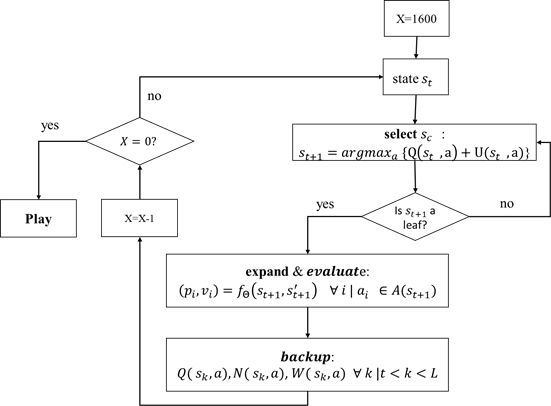
\includegraphics[scale=0.4]{a}
    \caption{Select: Each simulation traverses the tree by selecting the edge with
maximum action-value $Q$, plus an upper confidence bound $U$ that
depends on a stored prior probability $P$ and visit count $N$ for
that edge (which is incremented once traversed). Expand \& Evaluate:
The leaf node is expanded and the associated positions is evaluated
by the neural network $(P(s,\cdot),V(s))=f_{\theta}(s)$ ; the vector
of $P$ values are stored in the outgoing edges from $s$. Backup: Action-values
$Q$ are updated to track the mean of all evaluations $V$ in the
subtree below that action. play Once the search is complete, search
probabilities $\pi$ are returned, proportional to $N^{\frac{1}{\tau}}$,
where $N$ is the visit count of each move from the root state and
$\tau$ is a parameter controlling temperature.\label{fig:fig}}
\end{figure}


MCTS begins with a root node $s_0$. In training, the game tree is shared across
both players so it is most likely expanded. That is, has children. If playing,
then it is an empty tree. MCTS walks down the tree and selects for each state at
time $s_t$ an action $a_t$ where
\begin{equation}
a_t=\underset{a}{\text{argmax}}(Q(s_{t},a)+U(s_{t},a))\label{eq:1}
\end{equation}
and
\begin{equation}
U(s,a)=c_{\text{puct}}P(s,a)\frac{\sqrt{\sum_{b}N(s,b)}}{1+N(s,a)},\label{eq:2}
\end{equation}


The selection procedure is based on the following parameters stored
at each edge $(s,a)$ of the tree. The visit count $N(s,a)$, the
total action-value $W(s,a)$, the mean action-value $Q(s,a)$, and
the prior probability of selecting that edge $P(s,a)$ . These values
are stored for all legal actions $a\in A(s)$ from $s$.  where $c_{\text{puct}}$
is a constant determining the level of exploration.
Initially the visit counts are small numbers and the $U$ plays the
key role comparing to $Q$; the nodes with higher prior probability
are visited. However, this method asymptotically prefers actions with
high action-value. In other words, initially it explores more and
asymptotically it exploits more. 



Once the search reaches a
leaf node at time $L$ its children are added to the tree, with initial values

$$W(s_L, a_i) = 0, N(s_L, a_i) = 0, Q(s_L, a_i) = 0, P(s_L, a_i) = p_i$$

Then, all edges $t \leq L$ are updated with
$$N(s_t,a)=N(s_t,a)+1,W(s_t,a)=W(s_t,a)+v, Q(s_t,a)=\frac{W(s_t,a)}{N(s_t,a)}$$

Where $p$ and $v$ come from feeding the state through the network. Note here
that since we obtain a $v$ value for every call to the network, we replace $v$
with the average of all $v$ that we obtain.

If $s_L$ is a terminal node and cannot be expanded. All edges $t\leq L$ have
visit counts incremented and mean activation value adjusted
$Q(s_L,a)=\frac{W(s_L,a)}{N(s_L,a)}$. This procedure is done a fixed number of
times. Then $\pi$ is generated, where
$$\pi(a|s_0) = \frac{N(s_0,a)^{1/\tau}}{\sum_b N(s_0,b)^{1/\tau}}$$

Here $\tau$ is a temperature parameter. It is set to 1 for the first 30 moves of
the game, and then is set to be small, $\tau \rightarrow 0$. Again, this favors
exploration over exploitation earlier on in the game.


\subsection{Self play}
During training, at each iteration many games of self-play are generated. For
each move in each game, the tree maintained by MCTS is shared among both
players, since they are the same. Moves are sampled from the probabilities $\pi$
returned by the MCTS search. That is $a_t \tilde \pi$. After each iteration, the
network is trained based on the loss function
$$l=(z-v)^2 - \pi^T \log p$$
Note that we experimented with this loss function as $v$ is the average of $v$
for all forward operations.

\subsection{Evaluator}
At fixed iteration intervals in the training process, we evaluate the current
neural network, with the previous best $f_{\theta}^{\ast}$. When the two play
against each other, they do not share the game tree maintained by MCTS.
Moreover, the moves $a_t$ are not sampled from $\pi$ but instead

\begin{equation}
    a_t=\underset{a}{\text{argmax}} (\pi_t)
\end{equation}

If the player using the current network wins more than 55\% of the games, it is
used for subsequent iterations. If not, the previous best is used.

\subsection{Neural Network Architecture}

\section{Results}

\subsection{Performance}

Performance of the trained models was evaluated using the Elo\cit{Elo} rating system, the same measure used by the AlphaGo Zero paper. 

\section{Discussion}

\bibliography{references}
\bibliographystyle{IEEEtran}


\section{Author contributions}
\end{document}
